%% =============================================================================
%% CAPÍTULO: MARCO TEÓRICO
%% =============================================================================
\chapter{Marco Teórico}
\label{cap:marco-teorico}

Este capítulo presenta el marco teórico del trabajo, incluyendo los componentes
especializados disponibles en la plantilla para diferentes disciplinas.
Los componentes (definidos como \glspl{macro}) se cargan de forma modular
en el \gls{preambulo} para optimizar el tiempo de compilación.

Para usar los componentes, añade en el \gls{preambulo} del documento:

\begin{verbatim}
\usepackage[all]{eps-componentes}  % Todos los componentes
% o bien, solo los que necesites:
\usepackage[software,telecom]{eps-componentes}
\end{verbatim}

%% =============================================================================
\section{Componentes Comunes}
\label{sec:comp-comunes}

Los componentes comunes se cargan automáticamente y están disponibles para todas
las disciplinas. Proporcionan elementos visuales para destacar información,
organizar contenido y mejorar la legibilidad del documento.

%% -----------------------------------------------------------------------------
\subsection{Cajas de Información}
\label{subsec:cajas-info}

Cajas coloreadas para destacar diferentes tipos de mensajes. Cada tipo tiene un
color y un icono predefinido que transmite el propósito del contenido.

\minisec{Caja de información (infobox)}
Para notas informativas generales.

\begin{verbatim}
\begin{infobox}
  Contenido de la nota informativa.
\end{infobox}
\end{verbatim}

\begin{infobox}
  Esta es una caja de información general. Úsala para notas importantes
  o datos relevantes que el lector debe conocer.
\end{infobox}

\minisec{Caja de éxito (successbox)}
Para indicar que algo se ha completado correctamente o mostrar buenas prácticas.

\begin{verbatim}
\begin{successbox}
  Operación completada correctamente.
\end{successbox}
\end{verbatim}

\begin{successbox}
  Esta es una caja de éxito. Indica que algo se ha completado correctamente
  o muestra una buena práctica.
\end{successbox}

\minisec{Caja de advertencia (warningbox)}
Para alertar sobre algo que requiere atención pero no es crítico.

\begin{verbatim}
\begin{warningbox}
  Precaución: revisa este apartado antes de continuar.
\end{warningbox}
\end{verbatim}

\begin{warningbox}
  Esta es una caja de advertencia. Alerta sobre algo que requiere atención
  pero no es crítico.
\end{warningbox}

\minisec{Caja de peligro (dangerbox)}
Para indicar errores críticos o prácticas que deben evitarse.

\begin{verbatim}
\begin{dangerbox}
  ¡Peligro! Esta acción es irreversible.
\end{dangerbox}
\end{verbatim}

\begin{dangerbox}
  Esta es una caja de peligro. Indica un error crítico o algo que debe
  evitarse a toda costa.
\end{dangerbox}

\minisec{Caja de consejo (tipbox)}
Para ofrecer sugerencias útiles o trucos.

\begin{verbatim}
\begin{tipbox}
  Consejo: usa atajos de teclado para ser más eficiente.
\end{tipbox}
\end{verbatim}

\begin{tipbox}
  Esta es una caja de consejo. Ofrece sugerencias útiles o trucos
  para mejorar el trabajo.
\end{tipbox}

\minisec{Caja de nota (notebox)}
Para información adicional o comentarios secundarios.

\begin{verbatim}
\begin{notebox}
  Nota: este comportamiento puede variar según la configuración.
\end{notebox}
\end{verbatim}

\begin{notebox}
  Esta es una caja de nota. Para información adicional o comentarios
  secundarios.
\end{notebox}

%% -----------------------------------------------------------------------------
\subsection{Cajas con Título}
\label{subsec:cajas-titulo}

Cajas que permiten definir un encabezado personalizado para el contenido.

\minisec{Caja con título personalizado (titlebox)}
Caja genérica con título configurable.

\begin{verbatim}
\begin{titlebox}{Mi Título}
  Contenido de la caja con título personalizado.
\end{titlebox}
\end{verbatim}

\begin{titlebox}{Título Personalizado}
  Esta caja permite definir un título personalizado para el contenido.
  Es útil para destacar secciones específicas.
\end{titlebox}

\minisec{Caja de definición (definitionbox)}
Para definiciones formales de términos o conceptos.

\begin{verbatim}
\begin{definitionbox}{Término}
  Definición del término o concepto.
\end{definitionbox}
\end{verbatim}

\begin{definitionbox}{Algoritmo}
  Conjunto ordenado y finito de operaciones que permite hallar la
  solución de un problema.
\end{definitionbox}

\minisec{Caja de ejemplo (examplebox)}
Para mostrar ejemplos prácticos. El título es opcional.

\begin{verbatim}
\begin{examplebox}[Título opcional]
  Descripción del ejemplo práctico.
\end{examplebox}
\end{verbatim}

\begin{examplebox}[Ejemplo de uso]
  Aquí se muestra cómo aplicar el concepto explicado anteriormente
  en un caso práctico.
\end{examplebox}

\minisec{Caja de contenido importante (importantbox)}
Para destacar contenido que no debe pasarse por alto.

\begin{verbatim}
\begin{importantbox}
  Contenido especialmente importante.
\end{importantbox}
\end{verbatim}

\begin{importantbox}
  Este contenido es especialmente importante y no debe pasarse por alto
  durante la lectura del documento.
\end{importantbox}

%% -----------------------------------------------------------------------------
\subsection{Listas Especiales}
\label{subsec:listas}

Listas personalizadas para diferentes casos de uso: tareas, pros/contras y pasos.

\minisec{Lista de verificación (checklist)}
Para tareas o puntos de control con estados: completado, parcial o pendiente.

\begin{verbatim}
\begin{checklist}
  \item[\checked] Tarea completada
  \item[\partialchecked] Parcialmente completada
  \item[\unchecked] Tarea pendiente
\end{checklist}
\end{verbatim}

\begin{checklist}
  \item[\checked] Revisar documentación
  \item[\checked] Implementar funcionalidad básica
  \item[\partialchecked] Realizar pruebas unitarias
  \item[\unchecked] Desplegar en producción
\end{checklist}

\minisec{Lista de pros y contras (proscons)}
Para comparar ventajas e inconvenientes.

\begin{verbatim}
\begin{proscons}
  \pro Ventaja 1
  \pro Ventaja 2
  \con Desventaja 1
\end{proscons}
\end{verbatim}

\begin{proscons}
  \pro Fácil de implementar
  \pro Bien documentado
  \pro Comunidad activa
  \con Curva de aprendizaje inicial
  \con Requiere configuración adicional
\end{proscons}

\minisec{Lista de pasos (steplist)}
Para secuencias de acciones numeradas.

\begin{verbatim}
\begin{steplist}
  \step Primer paso
  \step Segundo paso
  \step Tercer paso
\end{steplist}
\end{verbatim}

\begin{steplist}
  \step Descargar el código fuente del repositorio
  \step Instalar las dependencias necesarias
  \step Configurar las variables de entorno
  \step Ejecutar el script de inicialización
  \step Verificar que todo funciona correctamente
\end{steplist}

%% -----------------------------------------------------------------------------
\subsection{Badges e Indicadores}
\label{subsec:badges}

Etiquetas visuales para marcar estados, versiones y métricas de progreso.

\minisec{Badge personalizado}
Etiqueta con texto y color personalizables. Colores disponibles: \texttt{eps-primary},
\texttt{eps-success}, \texttt{eps-warning}, \texttt{eps-danger}, \texttt{eps-secondary}.

\begin{verbatim}
\badge{Texto}                    % Color por defecto
\badge[eps-success]{Completado}  % Color específico
\end{verbatim}

\noindent
\badge{Estable} \quad
\badge[eps-success]{Completado} \quad
\badge[eps-warning]{En revisión} \quad
\badge[eps-danger]{Crítico} \quad
\badge[eps-secondary]{Beta}

\minisec{Badges predefinidos}
Atajos para estados comunes de desarrollo.

\begin{verbatim}
\badgenew \badgewip \badgedeprecated
\badgebeta \badgerequired \badgeoptional
\end{verbatim}

\noindent
\badgenew \quad \badgewip \quad \badgedeprecated \quad
\badgebeta \quad \badgerequired \quad \badgeoptional

\minisec{Indicador de versión}
Para mostrar números de versión con formato consistente.

\begin{verbatim}
\version{1.0.0} \version{2.1.0-beta}
\end{verbatim}

\noindent
\version{1.0.0} \quad \version{2.1.0} \quad \version{3.0.0-beta}

\minisec{Barra de progreso}
Indicador visual de porcentaje de completado (0-100).

\begin{verbatim}
\progressbar{25} \progressbar{75}
\end{verbatim}

\noindent
\progressbar{25} \quad \progressbar{50} \quad \progressbar{75} \quad \progressbar{100}

\minisec{Rating con estrellas}
Para valoraciones sobre un máximo.

\begin{verbatim}
\rating{3}{5}  % 3 de 5 estrellas
\end{verbatim}

\noindent
\rating{3}{5} \quad \rating{4}{5} \quad \rating{5}{5}

\minisec{Indicador de nivel}
Barras horizontales para representar niveles.

\begin{verbatim}
\levelbar{2}{5}  % Nivel 2 de 5
\end{verbatim}

\noindent
\levelbar{2}{5} \quad \levelbar{4}{5} \quad \levelbar{5}{5}

%% -----------------------------------------------------------------------------
\subsection{Tarjetas de Información}
\label{subsec:tarjetas}

Tarjetas compactas para mostrar información de personas o estadísticas.

\minisec{Tarjeta de persona (personcard)}
Para presentar miembros del equipo o colaboradores.

\begin{verbatim}
\personcard{Nombre}{Cargo}{Descripción breve}
\end{verbatim}

\noindent
\personcard{Juan García}{Desarrollador Senior}{%
  Especialista en arquitectura de software con 10 años de experiencia.%
}
\hfill
\personcard{María López}{Project Manager}{%
  Coordinación de equipos y gestión ágil de proyectos.%
}

\minisec{Tarjeta de estadística (statcard)}
Para métricas clave con icono y color. Requiere FontAwesome (\verb|\faIcono|).

\begin{verbatim}
\statcard{Valor}{Etiqueta}{\faIcono}{color}
\end{verbatim}

\vspace{1em}
\noindent
\statcard{1,234}{Usuarios}{\faUsers}{eps-primary}
\hfill
\statcard{98.5\%}{Uptime}{\faChartLine}{eps-success}
\hfill
\statcard{45ms}{Latencia}{\faClock}{eps-info}
\hfill
\statcard{12}{Issues}{\faBug}{eps-warning}

%% -----------------------------------------------------------------------------
\subsection{Timeline}
\label{subsec:timeline}

Línea temporal para representar secuencias de eventos cronológicos.

\begin{verbatim}
\begin{timeline}
  \timeitem{Fecha 1}{Descripción del evento 1}
  \timeitem{Fecha 2}{Descripción del evento 2}
\end{timeline}
\end{verbatim}

\begin{timeline}
  \timeitem{Ene 2024}{Inicio del proyecto y definición de requisitos}
  \timeitem{Mar 2024}{Diseño de la arquitectura del sistema}
  \timeitem{Jun 2024}{Implementación del módulo principal}
  \timeitem{Sep 2024}{Pruebas de integración y corrección de errores}
  \timeitem{Dic 2024}{Despliegue en producción y documentación final}
\end{timeline}

%% -----------------------------------------------------------------------------
\subsection{Comparativas}
\label{subsec:comparativas}

Tabla para comparar dos opciones lado a lado.

\begin{verbatim}
\begin{comparison}{Opción A}{Opción B}
  \comprow{Criterio 1}{Valor A}{Valor B}
  \comprow{Criterio 2}{Valor A}{Valor B}
\end{comparison}
\end{verbatim}

\begin{comparison}{Opción A}{Opción B}
  \comprow{Rendimiento}{Alto}{Medio}
  \comprow{Facilidad de uso}{Media}{Alta}
  \comprow{Coste}{Bajo}{Medio}
  \comprow{Soporte}{Comunidad}{Comercial}
\end{comparison}

%% -----------------------------------------------------------------------------
\subsection{Citas Destacadas}
\label{subsec:citas}

Bloque de cita con estilo visual destacado y atribución opcional.

\begin{verbatim}
\begin{quotebox}[Autor]
  Texto de la cita.
\end{quotebox}
\end{verbatim}

\begin{quotebox}[Albert Einstein]
  La imaginación es más importante que el conocimiento. El conocimiento
  es limitado, mientras que la imaginación abraza el mundo entero.
\end{quotebox}


%% =============================================================================
\section{Componentes de Software}
\label{sec:comp-software}

Componentes específicos para informática e ingeniería de software. Incluyen
documentación de APIs, terminales, estructuras de datos, diagramas UML y
control de versiones.

\begin{verbatim}
\usepackage[software]{eps-componentes}
\end{verbatim}

%% -----------------------------------------------------------------------------
\subsection{API REST Endpoints}
\label{subsec:api}

Documentación visual de endpoints de APIs REST con soporte para cuerpo de
petición y múltiples respuestas.

\begin{verbatim}
\begin{apiendpoint}{MÉTODO}{/ruta}
  Descripción del endpoint.

  \apibody{content-type}{cuerpo JSON}
  \apiresponse{código}{respuesta JSON}
\end{apiendpoint}
\end{verbatim}

\begin{apiendpoint}{GET}{/api/users}
  Obtiene la lista de todos los usuarios registrados en el sistema.
  Requiere autenticación mediante token JWT.

  \apibody{application/json}{
    "page": 1,
    "limit": 10,
    "filter": "active"
  }

  \apiresponse{200}{
    "users": [
      {"id": 1, "name": "Juan"},
      {"id": 2, "name": "María"}
    ],
    "total": 150
  }

  \apiresponse{401}{
    "error": "Token no válido"
  }
\end{apiendpoint}

\vspace{1em}

\begin{apiendpoint}{POST}{/api/users}
  Crea un nuevo usuario en el sistema.

  \apiresponse{201}{
    "id": 3,
    "message": "Usuario creado"
  }
\end{apiendpoint}

\minisec{Badges de métodos HTTP}
Etiquetas coloreadas para identificar métodos HTTP.

\begin{verbatim}
\httpget \httppost \httpput \httppatch \httpdelete
\end{verbatim}

\noindent
\httpget \quad \httppost \quad \httpput \quad \httppatch \quad \httpdelete

%% -----------------------------------------------------------------------------
\subsection{Terminal y Consola}
\label{subsec:terminal}

Simula una ventana de terminal con comandos de usuario normal y de root.

\begin{verbatim}
\begin{terminal}[Título opcional]
  \prompt comando de usuario
  \promptroot comando como root
\end{terminal}
\end{verbatim}

\begin{terminal}[Instalación de dependencias]
  \prompt npm install
  \prompt npm run build
  \prompt npm test
  \promptroot systemctl restart nginx
  \promptroot journalctl -u nginx -f
\end{terminal}

%% -----------------------------------------------------------------------------
\subsection{Árbol de Directorios}
\label{subsec:dirtree}

Representa la estructura de carpetas y archivos de un proyecto.

\begin{verbatim}
\begin{dirtreebox}[Título]
  \dirtreeitem[nivel]{nombre/}  % Carpeta
  \dirtreeitem[nivel]{archivo}  % Archivo
\end{dirtreebox}
\end{verbatim}

\begin{dirtreebox}[Estructura del Proyecto]
  \dirtreeitem[1]{src/}
  \dirtreeitem[2]{assets/}
  \dirtreeitem[3]{logo.png}
  \dirtreeitem[2]{components/}
  \dirtreeitem[3]{Header.js}
  \dirtreeitem[3]{Footer.js}
  \dirtreeitem[2]{App.js}
  \dirtreeitem[2]{index.js}
  \dirtreeitem[1]{package.json}
  \dirtreeitem[1]{README.md}
\end{dirtreebox}

%% -----------------------------------------------------------------------------
\subsection{Clases UML}
\label{subsec:uml}

Diagramas de clases e interfaces con notación UML estándar.

\minisec{Clase}
Define una clase con atributos y métodos. Usa \verb|\visibility{}| para indicar
visibilidad: \texttt{+} público, \texttt{-} privado, \texttt{\#} protegido.

\begin{verbatim}
\umlclass{NombreClase}{
  \visibility{-} atributo: tipo \\
}{
  \visibility{+} método(): tipo \\
}
\end{verbatim}

\umlclass{Usuario}{
  \visibility{-} id: int \\
  \visibility{-} nombre: string \\
  \visibility{-} email: string \\
  \visibility{#} password: string
}{
  \visibility{+} getNombre(): string \\
  \visibility{+} setNombre(n: string): void \\
  \visibility{+} validar(): boolean
}

\minisec{Interfaz}
Define una interfaz con sus métodos.

\begin{verbatim}
\umlinterface{NombreInterfaz}{
  \visibility{+} método(): tipo \\
}
\end{verbatim}

\umlinterface{IAutenticable}{
  \visibility{+} login(user: string, pass: string): boolean \\
  \visibility{+} logout(): void \\
  \visibility{+} isAuthenticated(): boolean
}

%% -----------------------------------------------------------------------------
\subsection{Tabla de Requisitos}
\label{subsec:requisitos}

Tabla para gestión de requisitos funcionales y no funcionales con prioridad y estado.

\begin{verbatim}
\begin{requirements}
  \requirement{ID}{Prioridad}{Estado}{Descripción}
\end{requirements}
\end{verbatim}

\begin{requirements}
  \requirement{RF-001}{Alta}{Completado}{El sistema debe permitir el registro de usuarios}
  \requirement{RF-002}{Alta}{Completado}{Los usuarios pueden modificar su perfil}
  \requirement{RF-003}{Media}{En progreso}{Implementar sistema de notificaciones}
  \requirement{RF-004}{Baja}{Pendiente}{Exportar datos a formato PDF}
  \requirement{RF-005}{Media}{Pendiente}{Integración con API externa}
\end{requirements}

%% -----------------------------------------------------------------------------
\subsection{Esquema de Base de Datos}
\label{subsec:database}

Documentación de tablas con claves primarias (\verb|\pkicon|) y foráneas (\verb|\fkicon|).

\begin{verbatim}
\begin{dbtable}{nombre_tabla}
  \pkicon & columna & TIPO & restricción \\
  \fkicon & columna & TIPO & FK -> tabla.columna \\
\end{dbtable}
\end{verbatim}

\begin{dbtable}{usuarios}
  \pkicon & id & INT & AUTO\_INCREMENT \\
  & nombre & VARCHAR(100) & NOT NULL \\
  & email & VARCHAR(255) & UNIQUE NOT NULL \\
  & created\_at & TIMESTAMP & DEFAULT NOW() \\
  \fkicon & rol\_id & INT & FK $\rightarrow$ roles.id \\
\end{dbtable}

\begin{dbtable}{roles}
  \pkicon & id & INT & AUTO\_INCREMENT \\
  & nombre & VARCHAR(50) & NOT NULL \\
  & permisos & JSON & NULL \\
\end{dbtable}

%% -----------------------------------------------------------------------------
\subsection{Git y Control de Versiones}
\label{subsec:git}

Elementos para documentar commits, ramas y etiquetas de Git.

\minisec{Commits}
Muestra un commit con hash, mensaje, autor y fecha.

\begin{verbatim}
\gitcommit{hash}{mensaje}{autor}{fecha}
\end{verbatim}

\gitcommit{a1b2c3d}{feat: Añadir sistema de autenticación}{Juan}{2024-01-15}
\gitcommit{e4f5g6h}{fix: Corregir error en validación de email}{María}{2024-01-20}
\gitcommit{i7j8k9l}{docs: Actualizar README con instrucciones}{Pedro}{2024-02-01}

\minisec{Ramas y etiquetas}
Badges para indicar ramas y versiones.

\begin{verbatim}
\gitbranch{nombre}  \gittag{versión}
\end{verbatim}

\noindent
\textbf{Ramas:} \gitbranch{main} \quad \gitbranch{develop} \quad \gitbranch{feature/login}

\vspace{0.5em}
\noindent
\textbf{Tags:} \gittag{v1.0.0} \quad \gittag{v1.1.0} \quad \gittag{v2.0.0-beta}

%% -----------------------------------------------------------------------------
\subsection{Logs y Métricas}
\label{subsec:logs}

Componentes para mostrar registros de eventos y métricas de rendimiento.

\minisec{Caja de logs (logbox)}
Muestra entradas de log con nivel, fecha y mensaje.

\begin{verbatim}
\begin{logbox}[Título]
  \logentry{NIVEL}{fecha hora}{mensaje}
\end{logbox}
\end{verbatim}

\begin{logbox}[Logs del servidor]
  \logentry{INFO}{2024-01-15 10:30:00}{Servidor iniciado en puerto 3000}
  \logentry{DEBUG}{2024-01-15 10:30:01}{Conexión a base de datos establecida}
  \logentry{WARN}{2024-01-15 10:35:22}{Intento de acceso sin autenticación}
  \logentry{ERROR}{2024-01-15 11:02:45}{Timeout en consulta a API externa}
\end{logbox}

\minisec{Tarjeta de métrica (metricbox)}
Muestra un valor con etiqueta, unidad y color indicador.

\begin{verbatim}
\metricbox{Etiqueta}{valor}{unidad}{color}
\end{verbatim}

\vspace{1em}
\noindent
\metricbox{Tiempo de respuesta}{45}{ms}{eps-success}
\hfill
\metricbox{Uso de CPU}{78}{\%}{eps-warning}
\hfill
\metricbox{Memoria}{2.4}{GB}{eps-info}


%% =============================================================================
\section{Componentes de Telecomunicaciones}
\label{sec:comp-telecom}

Componentes para telecomunicaciones, electrónica y sistemas de comunicación.
Incluyen diagramas de RF, tramas de protocolo, máquinas de estados y señales.

\begin{verbatim}
\usepackage[telecom]{eps-componentes}
\end{verbatim}

%% -----------------------------------------------------------------------------
\subsection{Carta de Smith}
\label{subsec:smith}

Herramienta gráfica para resolver problemas de adaptación de impedancias en
líneas de transmisión. Permite añadir trazados y puntos marcados.

\begin{verbatim}
\begin{smithchartbox}[Título]
  \addplot [...] coordinates {(r1,x1) (r2,x2)};
  \smithpoint{r}{x}{etiqueta}
\end{smithchartbox}
\end{verbatim}

\begin{smithchartbox}[Adaptación de Impedancias]
  \addplot [mark=none, eps-primary, thick] coordinates {(0.5,0.2) (0.2,0) (0.5,-0.2) (1,0)};
  \smithpoint{0.5}{0.2}{$Z_L$}
  \smithpoint{0.2}{0}{$Z_{in}$}
\end{smithchartbox}

%% -----------------------------------------------------------------------------
\subsection{Diagrama de Constelación}
\label{subsec:constelacion}

Representación gráfica de esquemas de modulación digital (QPSK, QAM, etc.).

\begin{verbatim}
\begin{constellationbox}[Título]
  \constpoint{I}{Q}{símbolo}
\end{constellationbox}
\end{verbatim}

\begin{constellationbox}[Constelación QPSK]
  \constpoint{1}{1}{00}
  \constpoint{-1}{1}{01}
  \constpoint{-1}{-1}{11}
  \constpoint{1}{-1}{10}
\end{constellationbox}

%% -----------------------------------------------------------------------------
\subsection{Máquina de Estados Finitos}
\label{subsec:fsm}

Diagramas FSM para representar autómatas y protocolos de comunicación.

\begin{verbatim}
\begin{fsmdiagram}
  \fsmstate{id}{x,y}{etiqueta}{opciones}  % opciones: initial
  \fsmtrans{origen}{destino}{etiqueta}
\end{fsmdiagram}
\end{verbatim}

\begin{fsmdiagram}
  \fsmstate{s0}{0,0}{IDLE}{initial}
  \fsmstate{s1}{3,0}{TX}{}
  \fsmstate{s2}{3,-2}{RX}{}
  \fsmtrans{s0}{s1}{start}
  \fsmtrans{s1}{s2}{ack}
  \fsmtrans{s2}{s0}{done}
\end{fsmdiagram}

%% -----------------------------------------------------------------------------
\subsection{Tramas de Protocolo}
\label{subsec:tramas}

Representación visual de tramas y paquetes de protocolos de comunicación.
Los campos con tamaño menor a 3 unidades muestran automáticamente su etiqueta
fuera del campo. Este umbral es configurable con \verb|\def\framenarrowthreshold{valor}|.

\minisec{Sintaxis básica}

\begin{verbatim}
\begin{protocolframe}[bits por fila]
  \framefield{bits}{etiqueta}      % Campo normal
  \framefieldvar[bits]{etiqueta}   % Campo de tamaño variable
  \framebreak                       % Salto de fila
\end{protocolframe}
\end{verbatim}

\minisec{Trama Ethernet IEEE 802.3}

\begin{protocolframe}[32]
  \framefield{7}{Preámbulo}
  \framefield{1}{SFD}
  \framefield{6}{MAC Dest}
  \framefield{6}{MAC Orig}
  \framefield{2}{Tipo}
  \framebreak
  \framefieldvar[32]{Datos (46-1500 bytes)}
  \framefield{4}{FCS}
\end{protocolframe}

\vspace{1em}

\minisec{Segmento TCP (cabecera simplificada)}

\begin{protocolframe}[16]
  \framefield{8}{Puerto Orig}
  \framefield{8}{Puerto Dest}
  \framefield{16}{Número Seq}
  \framefield{16}{Número ACK}
  \framefield{4}{Offset}
  \framefield{6}{Flags}
  \framefield{6}{Ventana}
  \framefield{8}{Checksum}
  \framefield{8}{Urg Ptr}
  \framebreak
  \framefieldvar[16]{Datos}
\end{protocolframe}

\vspace{1em}

\minisec{Campo multi-fila}
Para datos que ocupan varias filas consecutivas.

\begin{verbatim}
\framefieldmulti{filas}{bits}{etiqueta}
\end{verbatim}

\begin{protocolframe}[16]
  \framefield{4}{Version}
  \framefield{4}{IHL}
  \framefield{8}{TOS}
  \framefieldmulti{2}{16}{Payload (datos de usuario)}
  \framefield{16}{Checksum}
\end{protocolframe}

\vspace{1em}

\minisec{Campos con continuación}
Para campos que se dividen entre filas.

\begin{verbatim}
\framefieldstart{bits}{etiqueta}
\framefieldend{bits}{}
\end{verbatim}

\begin{protocolframe}[8]
  \framefield{4}{Ctrl}
  \framefieldstart{4}{Dirección}
  \framefieldend{2}{}
  \framefield{6}{Opciones}
  \framefield{8}{CRC}
\end{protocolframe}

\vspace{1em}

\minisec{Etiqueta externa forzada}
Fuerza la etiqueta fuera del campo, útil para campos estrechos.

\begin{verbatim}
\framefieldext{bits}{etiqueta}
\end{verbatim}

\begin{protocolframe}[16]
  \framefield{6}{Control}
  \framefieldext{2}{ID}
  \framefield{8}{Datos}
\end{protocolframe}

\vspace{1em}

\minisec{Campos reservados y agrupación}
Campos reservados con patrón rayado y llaves para agrupar filas.

\begin{verbatim}
\framefieldreserved{bits}          % Reservado
\framefieldreserved[texto]{bits}   % Con texto personalizado
\framefieldhighlight{bits}{texto}  % Campo destacado
\framewordgroup{fila_ini}{fila_fin}{etiqueta}
\end{verbatim}

\begin{protocolframe}[16]
  \framefield{4}{Ver}
  \framefield{4}{Tipo}
  \framefieldreserved{8}
  \framefield{8}{Longitud}
  \framefieldhighlight{8}{ID Sesión}
  \framefieldreserved[---]{16}
  \framewordgroup{0}{2}{Cabecera}
\end{protocolframe}

%% -----------------------------------------------------------------------------
\subsection{Parámetros S}
\label{subsec:sparams}

Tabla para especificaciones de parámetros de dispersión (S-parameters) en RF.

\begin{verbatim}
\begin{rfspecs}[Título]
  \rfspec{parámetro}{valor}{unidad}{descripción}
\end{rfspecs}
\end{verbatim}

\begin{rfspecs}[Parámetros S]
  \rfspec{$S_{11}$}{-18.5}{dB}{Pérdidas de retorno entrada}
  \rfspec{$S_{21}$}{-0.25}{dB}{Pérdidas de inserción}
  \rfspec{$S_{12}$}{-45.2}{dB}{Aislamiento inverso}
  \rfspec{$S_{22}$}{-22.1}{dB}{Pérdidas de retorno salida}
\end{rfspecs}

%% -----------------------------------------------------------------------------
\subsection{Diagramas de Bloques}
\label{subsec:bloques}

Diagramas de bloques para sistemas de RF, procesamiento de señales, etc.

\begin{verbatim}
\begin{blockdiagram}
  \sysblock{id}{x,y}{etiqueta}
  \sysarrow{origen}{destino}
\end{blockdiagram}
\end{verbatim}

\begin{blockdiagram}
  \sysblock{ant}{0,0}{Antena}
  \sysblock{lna}{3,0}{LNA}
  \sysblock{mix}{6,0}{Mixer}
  \sysblock{fil}{9,0}{Filtro}
  \sysarrow{ant}{lna}
  \sysarrow{lna}{mix}
  \sysarrow{mix}{fil}
\end{blockdiagram}

%% -----------------------------------------------------------------------------
\subsection{Diagramas de Temporización}
\label{subsec:timing}

Macros para dibujar diagramas de temporización de señales digitales.

\begin{verbatim}
\timingclock{x}{y}{ciclos}   % Señal de reloj
\timinglow{x}{y}{duración}   % Señal en bajo
\timinghigh{x}{y}{duración}  % Señal en alto
\end{verbatim}

\begin{center}
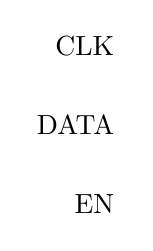
\begin{tikzpicture}
  % Señal de reloj
  \draw (0,2) node[left] {CLK};
  \timingclock{0}{2}{8}

  % Señal de datos
  \draw (0,1) node[left] {DATA};
  \timinglow{0}{1}{1}
  \timinghigh{1}{1}{2}
  \timinglow{3}{1}{1}
  \timinghigh{4}{1}{3}
  \timinglow{7}{1}{1}

  % Señal de enable
  \draw (0,0) node[left] {EN};
  \timinglow{0}{0}{2}
  \timinghigh{2}{0}{5}
  \timinglow{7}{0}{1}
\end{tikzpicture}
\end{center}


%% =============================================================================
\section{Componentes de Arquitectura}
\label{sec:comp-arquitectura}

Componentes para arquitectura, ingeniería civil y construcción. Incluyen
planificación, fichas técnicas, presupuestos, normativa y certificaciones.

\begin{verbatim}
\usepackage[arquitectura]{eps-componentes}
\end{verbatim}

%% -----------------------------------------------------------------------------
\subsection{Diagrama de Gantt}
\label{subsec:gantt}

Planificación temporal de proyectos con dependencias entre tareas.
Usa el paquete \texttt{pgfgantt} con estilo personalizado \texttt{eps gantt}.

\begin{verbatim}
\begin{ganttbox}[Título]
  \begin{ganttchart}[eps gantt, ...]{inicio}{fin}
    \gantttitle{Año}{meses} \\
    \ganttbar{Tarea}{inicio}{fin} \\
    \ganttlink{elem0}{elem1}
  \end{ganttchart}
\end{ganttbox}
\end{verbatim}

\begin{ganttbox}[Planificación de obra - Fase 1]
  \begin{ganttchart}[eps gantt, time slot format=simple, x unit=1.0cm]{1}{12}
    \gantttitle{Año 2024}{12} \\
    \gantttitle{E}{1}
    \gantttitle{F}{1}
    \gantttitle{M}{1}
    \gantttitle{A}{1}
    \gantttitle{M}{1}
    \gantttitle{J}{1}
    \gantttitle{J}{1}
    \gantttitle{A}{1}
    \gantttitle{S}{1}
    \gantttitle{O}{1}
    \gantttitle{N}{1}
    \gantttitle{D}{1} \\
    \ganttbar{Demolición}{1}{2} \\
    \ganttbar{Cimentación}{2}{4} \\
    \ganttbar[bar/.append style={fill=eps-danger}]{Estructura}{4}{8} \\
    \ganttbar{Cerramientos}{7}{10} \\
    \ganttbar{Instalaciones}{9}{12} \\
    \ganttlink{elem0}{elem1}
    \ganttlink{elem1}{elem2}
    \ganttlink{elem2}{elem3}
    \ganttlink{elem3}{elem4}
  \end{ganttchart}
\end{ganttbox}

%% -----------------------------------------------------------------------------
\subsection{Fichas Técnicas de Materiales}
\label{subsec:fichas-tecnicas}

Documentación de especificaciones técnicas de materiales de construcción.

\minisec{Ficha técnica completa (techsheet)}

\begin{verbatim}
\begin{techsheet}{Nombre del material}
  \techprop{Propiedad}{Valor}
\end{techsheet}
\end{verbatim}

\begin{techsheet}{Hormigón HA-25/B/20/IIa}
  \techprop{Resistencia característica}{25 MPa}
  \techprop{Consistencia}{Blanda (6-9 cm)}
  \techprop{Tamaño máximo árido}{20 mm}
  \techprop{Ambiente de exposición}{IIa - Humedad alta}
  \techprop{Relación agua/cemento máx.}{0.60}
  \techprop{Contenido mínimo cemento}{275 kg/m³}
  \techprop{Recubrimiento nominal}{30 mm}
\end{techsheet}

\minisec{Tarjeta compacta (materialcard)}

\begin{verbatim}
\materialcard{Nombre}{propiedades con \techprop{}{}}
\end{verbatim}

\vspace{1em}
\noindent
\materialcard{Acero B500S}{%
  \techprop{Límite elástico}{500 MPa}
  \techprop{Resistencia tracción}{550 MPa}
}
\hfill
\materialcard{Ladrillo cerámico}
}

%% -----------------------------------------------------------------------------
\subsection{Presupuestos}
\label{subsec:presupuesto}

Tabla de presupuesto con capítulos, partidas y cálculo automático de totales.

\begin{verbatim}
\begin{presupuesto}
  \capitulo{número}{NOMBRE}
  \partida{código}{descripción}{ud}{cantidad}{precio}
  \totalpresupuesto{importe}
\end{presupuesto}
\end{verbatim}

\begin{presupuesto}
  \capitulo{1}{MOVIMIENTO DE TIERRAS}
  \partida{1.1}{Excavación en zanjas}{m³}{120}{40}
  \partida{1.2}{Transporte a vertedero}{m³}{180}{15}
  \partida{1.3}{Compactación de tierras}{m²}{250}{4}
  \capitulo{2}{CIMENTACIÓN}
  \partida{2.1}{Hormigón de limpieza}{m³}{15}{80}
  \partida{2.2}{Zapatas de hormigón armado}{m³}{42}{300}
  \capitulo{3}{ESTRUCTURA}
  \partida{3.1}{Pilares de hormigón}{m³}{28}{400}
  \partida{3.2}{Forjado unidireccional}{m²}{320}{120}
  \totalpresupuesto{74660}
\end{presupuesto}

%% -----------------------------------------------------------------------------
\subsection{Normativa Aplicable}
\label{subsec:normativa}

Lista de normativa técnica aplicable al proyecto.

\begin{verbatim}
\begin{normativa}
  \norma{código}{descripción}{año}
\end{normativa}
\end{verbatim}

\begin{normativa}
  \norma{CTE DB-SE}{Seguridad Estructural - Bases de cálculo}{2019}
  \norma{CTE DB-SE-AE}{Acciones en la edificación}{2019}
  \norma{CTE DB-SE-C}{Cimientos}{2019}
  \norma{EHE-08}{Instrucción de Hormigón Estructural}{2008}
  \norma{UNE-EN 1992-1-1}{Eurocódigo 2: Proyecto de estructuras de hormigón}{2013}
  \norma{NCSE-02}{Norma de Construcción Sismorresistente}{2002}
\end{normativa}

%% -----------------------------------------------------------------------------
\subsection{Control de Calidad}
\label{subsec:control-calidad}

Tabla de resultados de ensayos con estado de conformidad (OK, PEND, NO).

\begin{verbatim}
\begin{controlcalidad}
  \controlitem{ensayo}{resultado}{especificación}{estado}
\end{controlcalidad}
\end{verbatim}

\begin{controlcalidad}
  \controlitem{\textbf{Hormigón HA-25}: Resistencia compresión}{28,5 MPa}{$\geq$ 25 MPa}{OK}
  \controlitem{\textbf{Acero B500S}: Límite elástico}{512 MPa}{$\geq$ 500 MPa}{OK}
  \controlitem{\textbf{Soldadura}: Inspección visual}{Defecto leve}{Sin defectos}{PEND}
  \controlitem{\textbf{Compactación}: Densidad relativa}{94\%}{$\geq$ 95\%}{NO}
\end{controlcalidad}

%% -----------------------------------------------------------------------------
\subsection{Etiquetas Energéticas}
\label{subsec:energia}

Etiquetas de calificación energética de edificios (A-G).

\begin{verbatim}
\etiquetaenergetica{letra}
\end{verbatim}

\noindent
\etiquetaenergetica{A} \quad
\etiquetaenergetica{B} \quad
\etiquetaenergetica{C} \quad
\etiquetaenergetica{D} \quad
\etiquetaenergetica{E} \quad
\etiquetaenergetica{F} \quad
\etiquetaenergetica{G}

%% -----------------------------------------------------------------------------
\subsection{Certificaciones}
\label{subsec:certificaciones}

Sellos de certificaciones ISO, marcado CE y normas UNE.

\begin{verbatim}
\certiso{número}    % ISO 9001, 14001, 45001...
\certce             % Marcado CE
\certune{número}    % Norma UNE
\end{verbatim}

\noindent
\certiso{9001} \quad \certiso{14001} \quad \certiso{45001}

\vspace{0.5em}
\noindent
\certce \quad \certune{12345}


%% =============================================================================
\section{Componentes de Química}
\label{sec:comp-quimica}

Componentes para química, ciencia de materiales e ingeniería química.
Incluyen reacciones, fichas de compuestos, protocolos y resultados analíticos.

\begin{verbatim}
\usepackage[quimica]{eps-componentes}
\end{verbatim}

%% -----------------------------------------------------------------------------
\subsection{Reacciones Químicas}
\label{subsec:reacciones}

Cajas para mostrar ecuaciones químicas con condiciones de reacción.
Usa el paquete \texttt{chemformula} para las fórmulas (\verb|\ch{}|).

\minisec{Caja de reacción (reactionbox)}

\begin{verbatim}
\begin{reactionbox}[Título]
  \ch{reactivos -> productos}
  \reactionconditions{temp}{presión}{catalizador}
\end{reactionbox}
\end{verbatim}

\begin{reactionbox}[Combustión completa del metano]
  \ch{CH4 + 2 O2 -> CO2 + 2 H2O}

  \reactionconditions{800\,\textdegree C}{1\,atm}{Pt}
\end{reactionbox}

\minisec{Caja de mecanismo (mechanismbox)}

\begin{verbatim}
\begin{mechanismbox}[Título]
  Descripción del mecanismo.
  \ch{ecuación}
\end{mechanismbox}
\end{verbatim}

\begin{mechanismbox}[Sustitución nucleofílica SN2]
  El mecanismo SN2 ocurre en un solo paso concertado donde el nucleófilo
  ataca por el lado opuesto al grupo saliente.

  \ch{HO^- + CH3Br -> CH3OH + Br^-}
\end{mechanismbox}

%% -----------------------------------------------------------------------------
\subsection{Fichas de Compuestos}
\label{subsec:compuestos}

Documentación de propiedades físico-químicas de compuestos.

\minisec{Ficha completa (compoundsheet)}

\begin{verbatim}
\begin{compoundsheet}{Nombre}{Fórmula}
  \compprop{propiedad}{valor}{unidad}
\end{compoundsheet}
\end{verbatim}

\begin{compoundsheet}{Ácido Sulfúrico}{H2SO4}
  \compprop{Masa molar}{98,079}{g/mol}
  \compprop{Densidad}{1,84}{g/cm³}
  \compprop{Punto de fusión}{10}{°C}
  \compprop{Punto de ebullición}{337}{°C}
  \compprop{Solubilidad en agua}{Miscible}{}
  \compprop{pKa}{-3 (ácido fuerte)}{}
\end{compoundsheet}

\minisec{Tarjeta compacta (compoundcard)}

\begin{verbatim}
\compoundcard{fórmula}{nombre}{masa molar}{descripción}
\end{verbatim}

\vspace{1em}
\noindent
\compoundcard{C2H5OH}{Etanol}{46,07 g/mol}{Líquido volátil}
\hfill
\compoundcard{C6H12O6}{Glucosa}{180,16 g/mol}{Sólido cristalino}

%% -----------------------------------------------------------------------------
\subsection{Protocolos de Laboratorio}
\label{subsec:protocolos}

Procedimientos de laboratorio con pasos numerados y advertencias.

\begin{verbatim}
\begin{protocol}[Título]
  \protocolstep{Paso a realizar}
  \protocolwarning{Advertencia de seguridad}
\end{protocol}
\end{verbatim}

\begin{protocol}[Titulación ácido-base]
  \protocolstep{Lavar y enjuagar la bureta con la solución valorante (\ch{NaOH} 0,1 M)}
  \protocolstep{Llenar la bureta y enrasar a cero}
  \protocolstep{Pipetear 25 mL de la muestra ácida en un erlenmeyer}
  \protocolstep{Añadir 3-4 gotas de indicador fenolftaleína}
  \protocolstep{Valorar hasta viraje de incoloro a rosa persistente}
  \protocolwarning{Usar gafas de seguridad y bata en todo momento}
  \protocolstep{Anotar el volumen gastado y repetir 3 veces}
\end{protocol}

%% -----------------------------------------------------------------------------
\subsection{Resultados Analíticos}
\label{subsec:analiticos}

Tabla de resultados analíticos con incertidumbre y código de color.

\begin{verbatim}
\begin{analyticalresults}
  \analyte{nombre}{valor}{incert}{unidad}{color}
\end{analyticalresults}
\end{verbatim}

\begin{analyticalresults}
  \analyte{Plomo (Pb)}{0,015}{0,001}{mg/L}{eps-danger}
  \analyte{Cadmio (Cd)}{0,002}{0,0005}{mg/L}{eps-success}
  \analyte{Mercurio (Hg)}{0,0005}{0,0001}{mg/L}{eps-success}
  \analyte{Arsénico (As)}{0,008}{0,002}{mg/L}{eps-success}
  \analyte{Cobre (Cu)}{0,85}{0,05}{mg/L}{eps-success}
  \analyte{Zinc (Zn)}{2,3}{0,1}{mg/L}{eps-warning}
\end{analyticalresults}

%% -----------------------------------------------------------------------------
\subsection{Equipamiento de Laboratorio}
\label{subsec:equipamiento}

Listas de equipos e inventario de reactivos para documentar el material usado.

\minisec{Lista de equipos (equipmentlist)}

\begin{verbatim}
\begin{equipmentlist}
  \item Nombre del equipo (modelo)
\end{equipmentlist}
\end{verbatim}

\begin{equipmentlist}
  \item Espectrofotómetro UV-Vis (Shimadzu UV-1800)
  \item pH-metro digital (Mettler Toledo)
  \item Balanza analítica (precisión 0,0001 g)
  \item Agitador magnético con calefacción
  \item Campana de extracción de gases
\end{equipmentlist}

\minisec{Lista de reactivos (reagentlist)}

\begin{verbatim}
\begin{reagentlist}
  \reagent{nombre}{concentración}{cantidad}{proveedor}
\end{reagentlist}
\end{verbatim}

\begin{reagentlist}
  \reagent{NaOH}{0,1 M}{500 mL}{Panreac}
  \reagent{HCl}{0,1 M}{250 mL}{Sigma-Aldrich}
  \reagent{"Fenolftaleína"}{1\% en etanol}{100 mL}{Scharlau}
  \reagent{"Agua destilada"}{--}{2 L}{Laboratorio}
\end{reagentlist}


%% =============================================================================
\section{Componentes de Geología}
\label{sec:comp-geologia}

Componentes para geología, geotecnia e ingeniería geológica. Incluyen
columnas estratigráficas, tablas de minerales, datos geotécnicos y simbología.

\begin{verbatim}
\usepackage[geologia]{eps-componentes}
\end{verbatim}

%% -----------------------------------------------------------------------------
\subsection{Columna Estratigráfica}
\label{subsec:estratigrafia}

Representación gráfica de secuencias de capas geológicas.

\begin{verbatim}
\begin{stratigraphybox}[Título]
  \begin{stratcolumn}
    \stratlayer{espesor}{patrón}{nombre}{edad}
  \end{stratcolumn}
\end{stratigraphybox}
\end{verbatim}

\begin{stratigraphybox}[Sección estratigráfica A-A']
    \begin{stratcolumn}
      \stratlayer{1}{lito arenisca}{Arenisca calcárea}{(Mioceno)}
      \stratlayer{1}{lito arcilla}{Margas grises}{(Mioceno)}
      \stratlayer{2}{lito caliza}{Caliza masiva}{(Cretácico)}
      \stratlayer{2}{lito dolomia}{Dolomías tableadas}{(Jurásico)}
    \end{stratcolumn}
\end{stratigraphybox}

%% -----------------------------------------------------------------------------
\subsection{Tabla de Minerales}
\label{subsec:minerales}

Tablas y tarjetas para documentar propiedades mineralógicas.

\minisec{Tabla de minerales (mineraltable)}

\begin{verbatim}
\begin{mineraltable}
  \mineralrow{nombre}{dureza}{densidad}{-}{-}{fórmula}
\end{mineraltable}
\end{verbatim}

\begin{mineraltable}
  \mineralrow{Cuarzo}{7}{2,65}{--}{--}{SiO2}
  \mineralrow{Calcita}{3}{2,71}{--}{--}{CaCO3}
  \mineralrow{Feldespato potásico}{6}{2,56}{--}{--}{KAlSi3O8}
  \mineralrow{Moscovita}{2,5}{2,82}{--}{--}{KAl2(AlSi3O10)(OH)2}
  \mineralrow{Olivino}{6,5}{3,32}{--}{--}{(Mg,Fe)2SiO4}
\end{mineraltable}

\minisec{Tarjeta de mineral (mineralcard)}

\begin{verbatim}
\mineralcard{nombre}{fórmula}{sistema}{dureza}{uso}
\end{verbatim}

\vspace{1em}
\noindent
\mineralcard{Pirita}{FeS2}{Cúbico}{6-6.5}{Ácido sulfúrico}
\hfill
\mineralcard{Galena}{PbS}{Cúbico}{2.5}{Mena de plomo}

%% -----------------------------------------------------------------------------
\subsection{Datos Geotécnicos}
\label{subsec:geotecnia}

Tablas de ensayos geotécnicos y comandos para valores característicos.

\minisec{Tabla de ensayos (geotechdata)}

\begin{verbatim}
\begin{geotechdata}
  \geotechtest{ensayo}{símbolo}{valor}{unidad}{norma}
\end{geotechdata}
\end{verbatim}

\begin{geotechdata}
  \geotechtest{Límite líquido}{LL}{45,2}{\%}{--}
  \geotechtest{Límite plástico}{LP}{23,1}{\%}{--}
  \geotechtest{Índice de plasticidad}{IP}{22,1}{\%}{--}
  \geotechtest{Densidad seca}{$\rho_d$}{1,72}{g/cm³}{--}
  \geotechtest{Humedad natural}{$w$}{18,5}{\%}{--}
\end{geotechdata}

\minisec{Valores característicos}

\begin{verbatim}
\sptvalue{golpes}   \cohesion{kPa}   \friction{grados}
\end{verbatim}

\vspace{0.5em}
\noindent
Ensayo SPT: \sptvalue{18} \quad
Cohesión: \cohesion{25} \quad
Ángulo de rozamiento: \friction{32}

%% -----------------------------------------------------------------------------
\subsection{Clasificación de Suelos}
\label{subsec:clasificacion-suelos}

Etiquetas USCS y clasificación RMR de macizos rocosos.

\begin{verbatim}
\uscsclass{código}          % USCS (CL, SM, GP, etc.)
\rmrclass{puntos}{clase}    % RMR (I-V)
\end{verbatim}

\noindent
Según el Sistema Unificado de Clasificación de Suelos (USCS):

\noindent
\uscsclass{CL} -- Arcilla de baja plasticidad

\noindent
\uscsclass{SM} -- Arena limosa

\noindent
\uscsclass{GP} -- Grava mal graduada

\vspace{1em}
\noindent
Clasificación RMR del macizo rocoso: \rmrclass{50}{III}

%% -----------------------------------------------------------------------------
\subsection{Eras Geológicas}
\label{subsec:eras}

Etiquetas para indicar periodos geológicos.

\begin{verbatim}
\geoera{nombre}
\end{verbatim}

\noindent
\geoera{Cuaternario} \quad
\geoera{Neógeno} \quad
\geoera{Paleógeno} \quad
\geoera{Cretácico} \quad
\geoera{Jurásico}

%% -----------------------------------------------------------------------------
\subsection{Riesgos Geológicos}
\label{subsec:riesgos-geo}

Indicadores de riesgos geológicos con nivel y descripción.

\begin{verbatim}
\georisk{nivel}{descripción}{color}
\risklandslide  \riskflood  \riskseismic
\end{verbatim}

\georisk{Riesgo Nivel 4}{Deslizamientos activos en ladera norte}{eps-danger}
\georisk{Riesgo Nivel 2}{Riesgo moderado de subsidencia}{eps-warning}

\vspace{0.5em}
\noindent
\risklandslide \quad \riskflood \quad \riskseismic

%% -----------------------------------------------------------------------------
\subsection{Símbolos Geológicos}
\label{subsec:simbolos-geo}

Símbolos estándar para mapas y cortes geológicos.

\begin{verbatim}
\faultline      \anticline   \syncline        \strikeanddip
\verticalbeds   \horizontalbeds
\end{verbatim}

\begin{center}
\begin{tabular}{c c c c}
  \faultline & \anticline & \syncline & \strikeanddip \\
  Falla & Anticlinal & Sinclinal & Rumbo/Buzamiento \\[1em]
  \verticalbeds & \horizontalbeds & & \\
  Estratos Vert. & Estratos Horiz. & & \\
\end{tabular}
\end{center}


%% =============================================================================
\section{Componentes de Prevención}
\label{sec:comp-prevencion}

Componentes para prevención de riesgos laborales y seguridad. Incluyen
matrices de riesgo, evaluaciones, señalización, EPIs y documentación.

\begin{verbatim}
\usepackage[prevencion]{eps-componentes}
\end{verbatim}

%% -----------------------------------------------------------------------------
\subsection{Matriz de Riesgos}
\label{subsec:matriz-riesgos}

Matriz 5×5 de probabilidad vs severidad para evaluación de riesgos.

\begin{verbatim}
\begin{riskmatrixbox}[Título]
  \riskmatrix
\end{riskmatrixbox}
\end{verbatim}

\begin{riskmatrixbox}[Matriz de evaluación 5×5]
  \riskmatrix
\end{riskmatrixbox}

%% -----------------------------------------------------------------------------
\subsection{Evaluación de Riesgos}
\label{subsec:evaluacion-riesgos}

Tabla para documentar riesgos identificados con probabilidad, severidad y medidas.

\begin{verbatim}
\begin{riskassessment}
  \riskentry{ID}{descripción}{prob}{sev}{}{medidas}
\end{riskassessment}
\end{verbatim}

\begin{riskassessment}
  \riskentry{R-001}{Caída a distinto nivel (andamios)}{4}{4}{}{Instalación de barandillas, redes de seguridad}
  \riskentry{R-002}{Contacto eléctrico directo}{2}{5}{}{Revisión periódica de instalaciones}
  \riskentry{R-003}{Golpes por objetos móviles}{3}{3}{}{Señalización de zonas de paso}
  \riskentry{R-004}{Sobreesfuerzos}{4}{2}{}{Formación en manipulación manual de cargas}
  \riskentry{R-005}{Exposición a ruido}{3}{2}{}{Uso obligatorio de protección auditiva}
\end{riskassessment}

%% -----------------------------------------------------------------------------
\subsection{Checklist de Seguridad}
\label{subsec:checklist-seguridad}

Lista de verificación con estados: completado, pendiente o no aplica.

\begin{verbatim}
\begin{safetychecklist}[Título]
  \checkitem{Punto verificado}
  \uncheckitem{Punto pendiente}
  \naitem{No aplica}
\end{safetychecklist}
\end{verbatim}

\begin{safetychecklist}[Verificación diaria de obra]
  \checkitem{EPIs disponibles y en buen estado}
  \checkitem{Zona de trabajo correctamente señalizada}
  \checkitem{Extintores accesibles y revisados}
  \uncheckitem{Revisión de andamios completada}
  \uncheckitem{Botiquín de primeros auxilios revisado}
  \naitem{Trabajos en espacios confinados}
\end{safetychecklist}

%% -----------------------------------------------------------------------------
\subsection{Señalización de Seguridad}
\label{subsec:senalizacion}

Señales de seguridad según normativa: advertencia, prohibición, obligación y emergencia.

\begin{verbatim}
\signwarning{texto}     % Advertencia (amarillo)
\signprohibition{texto} % Prohibición (rojo)
\signmandatory{texto}   % Obligación (azul)
\signemergency{texto}   % Emergencia (verde)
\signfire{texto}        % Extinción (rojo)
\end{verbatim}

\minisec{Señales de advertencia}
\signwarning{Riesgo de caída a distinto nivel}
\signwarning{Riesgo eléctrico}

\minisec{Señales de prohibición}
\signprohibition{Prohibido fumar}
\signprohibition{Prohibido el paso}

\minisec{Señales de obligación}
\signmandatory{Uso obligatorio de casco}
\signmandatory{Uso obligatorio de guantes}

\minisec{Señales de emergencia}
\signemergency{Salida de emergencia}
\signfire{Extintor}

%% -----------------------------------------------------------------------------
\subsection{Equipos de Protección Individual}
\label{subsec:epis}

Iconos de EPIs para listas de equipamiento obligatorio.

\begin{verbatim}
\begin{epilist}
  \item \epihardhat      % Casco
  \item \epigloves       % Guantes
  \item \epigoggles      % Gafas
  \item \epiboots        % Botas
  \item \epimask         % Mascarilla
  \item \epiearprotection % Protección auditiva
  \item \epivest         % Chaleco
  \item \epiharness      % Arnés
\end{epilist}
\end{verbatim}

\begin{epilist}
  \item \epihardhat
  \item \epigloves
  \item \epigoggles
  \item \epiboots
  \item \epimask
  \item \epiearprotection
  \item \epivest
  \item \epiharness
\end{epilist}

%% -----------------------------------------------------------------------------
\subsection{Indicadores de Seguridad}
\label{subsec:indicadores-seguridad}

Índices de siniestralidad y contador de días sin accidentes.

\begin{verbatim}
\indicatorIF{valor}       % Índice de frecuencia
\indicatorIG{valor}       % Índice de gravedad
\indicatorII{valor}       % Índice de incidencia
\indicatorDaysSafe{días}  % Días sin accidentes
\end{verbatim}

\noindent
\indicatorIF{12,5}
\hfill
\indicatorIG{0,35}
\hfill
\indicatorII{8,2}
\hfill
\indicatorDaysSafe{247}

%% -----------------------------------------------------------------------------
\subsection{Procedimiento de Emergencia}
\label{subsec:emergencia}

Protocolo de actuación con pasos y teléfonos de emergencia.

\begin{verbatim}
\begin{emergencyprocedure}[Título]
  % Contenido (puede usar steplist)
  \emergencyphone{nombre}{teléfono}
\end{emergencyprocedure}
\end{verbatim}

\begin{emergencyprocedure}[En caso de accidente grave]
  \begin{steplist}
    \step Proteger: Asegurar la zona y evitar nuevos accidentes
    \step Avisar: Llamar al 112 y comunicar a los servicios de emergencia
    \step Socorrer: Aplicar primeros auxilios si se tiene formación
    \step No mover al accidentado salvo peligro inminente
    \step Esperar a los servicios de emergencia
  \end{steplist}

  \vspace{0.5em}
  \emergencyphone{Emergencias}{112}\\
  \emergencyphone{Mutua de accidentes}{900 123 456}\\
  \emergencyphone{Responsable de seguridad}{ext. 2345}
\end{emergencyprocedure}

%% -----------------------------------------------------------------------------
\subsection{Registro de Formación}
\label{subsec:formacion}

Registro de formación en prevención con estado de vigencia.

\begin{verbatim}
\begin{trainingrecord}
  \trainingentry{curso}{horas}{fecha}{caducidad}{estado}
  % estado: vigente, proximo, caducado
\end{trainingrecord}
\end{verbatim}

\begin{trainingrecord}
  \trainingentry{PRL Básico (60h)}{60}{01/2024}{01/2029}{vigente}
  \trainingentry{Trabajos en altura}{8}{03/2024}{03/2025}{vigente}
  \trainingentry{Primeros auxilios}{16}{06/2023}{06/2025}{proximo}
  \trainingentry{Riesgo eléctrico}{20}{01/2022}{01/2024}{caducado}
\end{trainingrecord}

%% -----------------------------------------------------------------------------
\subsection{Informe de Accidente}
\label{subsec:accidente}

Formulario estructurado para documentar accidentes laborales.

\begin{verbatim}
\begin{accidentreport}[Título]
  \reportfield{Campo}{Valor}
  \reportfield{Gravedad}{\accidenttype{leve|grave|muy grave}}
\end{accidentreport}
\end{verbatim}

\begin{accidentreport}[Informe de accidente laboral]
  \reportfield{Fecha}{15 de enero de 2024}
  \reportfield{Hora}{10:30}
  \reportfield{Lugar}{Zona de carga, nave 3}
  \reportfield{Trabajador}{Juan García Pérez}
  \reportfield{Tipo de lesión}{Contusión en pie derecho}
  \reportfield{Gravedad}{\accidenttype{leve}}
  \reportfield{Descripción}{Caída de caja desde estantería sobre el pie}
  \reportfield{Causa principal}{Almacenamiento inadecuado de materiales}
  \reportfield{Medidas correctoras}{Revisión del sistema de almacenamiento}
\end{accidentreport}
